\documentclass[fleqn, 12.5pt,a4paper]{report}
\usepackage{amsmath,amssymb}
\usepackage{nccmath}
\usepackage{subfig}
\usepackage[utf8]{inputenc}
\usepackage[nottoc]{tocbibind}
\usepackage[dvipsnames]{xcolor}
\usepackage[colorlinks,citecolor=green,urlcolor=blue,bookmarks=true,hypertexnames=true]{hyperref}
\usepackage[a4paper, total={7in, 9in}]{geometry}
\usepackage{xcolor}
\usepackage{caption}
\usepackage{subcaption}
\usepackage{amsmath}
\usepackage{color}   %May be necessary if you want to color links
\usepackage[colorlinks,citecolor=green,urlcolor=blue,bookmarks=true,hypertexnames=true]{hyperref}
\usepackage{lipsum}
\usepackage[english]{babel}
\usepackage{bigints}
\usepackage{sectsty}
\newcommand\tab[1][1cm]{\hspace*{#1}}
\usepackage{fixmath}
\usepackage{physics}
\usepackage[mathscr]{euscript}
\usepackage{tabularx}
\usepackage{fancyhdr}
\pagestyle{fancy}
\usepackage[mathscr]{euscript}
\usepackage{graphicx}
\usepackage{float}
\newcommand{\colvec}[2][.8]{%
  \scalebox{#1}{%
    \renewcommand{\arraystretch}{.8}%
    $\begin{bmatrix}#2\end{bmatrix}$%
  }
}
\fancyhf{}
\fancyhead[RE,LO]{XFEM and LEFM}
\fancyfoot[RE,LO]{Vikas Melkot Balasubramanyam}
\fancyfoot[LE,RO]{\thepage}
\newcommand{\uls}[1]{\mskip.5\thinmuskip\underline{\mskip-.5\thinmuskip {#1} \mskip-.5\thinmuskip}\mskip.5\thinmuskip} % underline short
\renewcommand{\headrulewidth}{2pt}
\renewcommand{\footrulewidth}{1pt}
\usepackage[T1]{fontenc}
\usepackage{euler}
\hypersetup{
    colorlinks=true, %set true if you want colored links
    linktoc=all,     %set to all if you want both sections and subsections linked
    linkcolor=blue,  %choose some color if you want links to stand out
}
%\usepackage{chngcntr}
\counterwithout{section}{chapter}
\renewcommand{\baselinestretch}{1.5}
\usepackage{setspace}
\title{Abstract_Introduction}
\author{Vikas Mb}
\date{February 2022}
\doublespacing

\begin{document}
\include{./Title}
\tableofcontents
\listoffigures
\newpage

\section{\color{Black} \large{Abstract}}
A new and improved technique called Extended Finite Element Method (XFEM) for modelling of cracks in the finite element framework has been presented. Standard displacements are enriched near a crack by incorporating both discontinuous fields and the near tip asymptotic fields through a partition of unity method\cite{khoei2014extended}. \par
\vspace{0.25cm}
The nodes that are present around the crack segments will be enriched giving rise to additional degree of freedoms. These additional DOFs are used to approximate displacements of the corresponding nodes. Displacements and stresses are computed after solving a BVP. \par 
\vspace{0.25cm}
The output from the XFEM will be used as the inputs to interaction integral to compute stress intensity factor. Finally, the crack is allowed to propagate. Numerical experiments are provided to demonstrate the correctness and robustness of the implemented technique.

\section{\color{Black} \large{Introduction}}
History has witnessed numerous scenarios of structural failure due to existence of cracks. Buildings, dams, bridges, airplanes, railroads, and many other constructions have been impacted with this phenomenon that has the catastrophic effects in the world\cite{kuna2013finite}. \par
\vspace{0.25cm}
Many scientists and engineers have come with the solutions and strategies to decrease the effects of cracks and prevent their occurrences in the structures. 
One can establish an analytical solution for simple cases. The real-life problems encountered in this front require complex solutions that can be obtained by computational techniques\cite{kuna2013finite}. The Finite element method plays a vital role in this regard. However, it is difficult to model the cracks (discontinuities in the displacements) as accurately as possible using this technique. \par
\vspace{0.25cm}
In order to model these discontinuities and inaccuracies the extended finite element method (XFEM) was developed in 1999 by Ted Belytschko\cite{belytschko1999elastic}.

\subsection{\color{Black} {Advantages of XFEM over standard FEM}}
\begin{itemize}
    \item Unlike FEM, this method captures the discontinuities in the displacements due to the presence of cracks accurately\cite{khoei2014extended}.
    \item This technique allows the entire crack to be represented independently of the mesh, and so re-meshing is not necessary to model crack growth\cite{khoei2014extended}.
    \item Computational effort is significantly less compared to usual FEM.
\end{itemize}

\section{\color{Black} \large{Partition of Unity Finite Element Method, PU-FEM}}  
A Partition of Unity can be defined as a collection of global functions $f_i(x)$ whose support is contained in a cloud and whose value sum to unity at each point x in the solution domain as \cite{ahmed2009extended}
$$\sum_{i=1}^N f_i(x) = 1, \hspace{0.25cm} \forall {x\in \Omega} $$ 

By choosing an arbitrary function $\psi(x)$ defined on domain $\Omega^{PU}$, the following property can be observed as\cite{khoei2014extended}

$$\sum_{i=1}^N f_i(x) \psi(x_i) = \psi(x)$$

In the FE approach, the shape functions are usually represented as a PU-FEM. Based on the concept of the PU-FEM, the displacement field $u(x)$ can be discretized over the domain of the problem \cite{khoei2014extended} by taking $f_i(x) \equiv N_i(x)$ as

$$\textbf{u($x$)} = \sum_{i=1}^{\mathscr{N}} N_i(x) u_i$$

wherein ${\mathscr{N}}$ is the number of nodal points for each finite element and $N_i(x)$ is the standard FEM shape function.

The incorporation of local enrichment to approximate displacement was originally introduced by Melenk and Babuška (1996) through the PU FEM \cite{ahmed2009extended}. The essential feature is based on the multiplication of enrichment functions by nodal shape functions\cite{ahmed2009extended}.It should be noted that only certain nodes are selected for the enrichment and the FE approximation of enriched domain takes the form

$$u(x) = \sum_{I\in \mathscr{N}} N_I(x) u_I + \sum_{J\in \mathscr{N}^{enr}} N_J(x)\psi(x) u_J $$ 

Expanding the above equation leads to

$$u(x) = \sum_{i=1}^n N_i(x) u_i + \sum_{j^{heavy}=1}^P N_j(x)[\psi(x)] a_j + \sum_{k^{tip}=1}^4 N_k(x)[\beta_{\alpha}(x)] b_{k^\alpha} $$\newline

wherein, $H(x)$ is the Heaviside function, $a_j$ are the additional degree of freedoms
associated with Heaviside jump function, $\beta(x)$ represents the branch function and $b_k$ are the additional degree of freedoms associated with branch function and $\alpha$ takes the values from 1 to 4 for each node\cite{khoei2014extended}.

\section{\color{Black} \large{Extended Finite Element Method (XFEM) - Realization in 2D}}
Extended finite element method is a partition of unity based method which helps us to model discontinuities that are arbitrarily aligned with the mesh. The main idea behind XFEM is, to enrich the crack containing elements using enrichment functions in standard finite element framework\cite{ahmed2009extended}.\newline 

In this project, Heaviside step function and Asymptotic branch functions have been used as the extrinsic enrichment functions for the displacement approximation\cite{ahmed2009extended} . The method entails selection of enriched nodes and elements, a usual FEM procedure such as defining the quadratic shape functions, defining the Iso-parametric elements, converting local coordinate system to global coordinate system using Jacobin matrix, computing, strain-displacement matrix, applying Gauss type integration method, and generating element stiffness matrix. All the necessary steps that are required to solve a BVP using XFEM will be discussed in the following sub-sections.

\subsection{\color{Black} {Selection of enriched nodes and elements}}
It has been assumed that the cracks propagate through the elements \cite{belytschko1999elastic} hence, it is very important to identify properly the elements and nodes that are to be enriched. If an element is completely cut by the crack [12,13,19,18] as shown in the figure, then that element should be enriched using Heaviside step function\cite{khoei2014extended}.

On the other hand, should the element [14,15,21,20] contains the crack tip, then the corresponding element should be enriched using Asymptotic branch functions\cite{pandey2019new}. The element [13,14,20,19] which is lying exactly behind the crack tip containing element, will have mixed enrichment\cite{khoei2014extended}. It means that the element will be enriched using both Heaviside and Asymptotic branch functions.

\subsection{\color{Black} {Selection of Blended elements}}
In the below illustration, all the elements that are surrounding the crack containing elements will be considered as the blended elements\cite{khoei2014extended}. These elements share their nodes with the enriched elements. The shared nodes will also be enriched accordingly. The blended elements could have 12, 18 and 24 DOFs. This includes 8 normal DOFs and the rest are considered to be the additional DOFs. 

\subsection{\color{Black} {Selection of Mixed Enriched elements}}
In the below illustration, node no [13,14,20,19] should be mixed enriched because Node numbers [14,20] are sharing their positions with the next element [14,15,21,20] which is Tip enriched and [13,19] are sharing their positions with the element [12,13,19,18] which is completely Heaviside enriched. Hence, node numbers [13,19] will be Heaviside enriched and node numbers [14,20] will be Tip enriched. This type of elements could have 22,28,34 degree of freedoms that leads to a element stiffness matrix of 22x22, 28x28 and 34x34.

%[width = 11cm,height =11cm]
\begin{figure}[H]
  \centering
  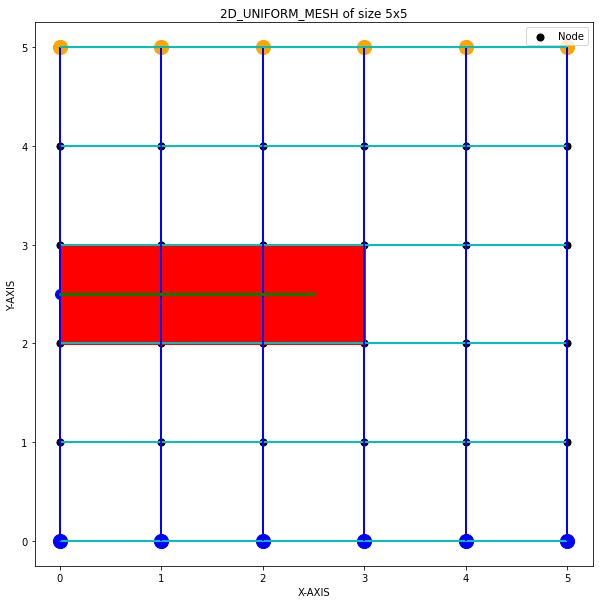
\includegraphics[scale=0.4]{enriched.png}
  \centering
  \textbf{\caption{Elements selected for the enrichment}}
\end{figure}

\begin{figure}[h]
  \centering
  \includegraphics[scale=0.4]{Blend.png}
  \centering
  \textbf{\caption{Blended-elements}}
\end{figure}

\begin{figure}[H]
  \centering
  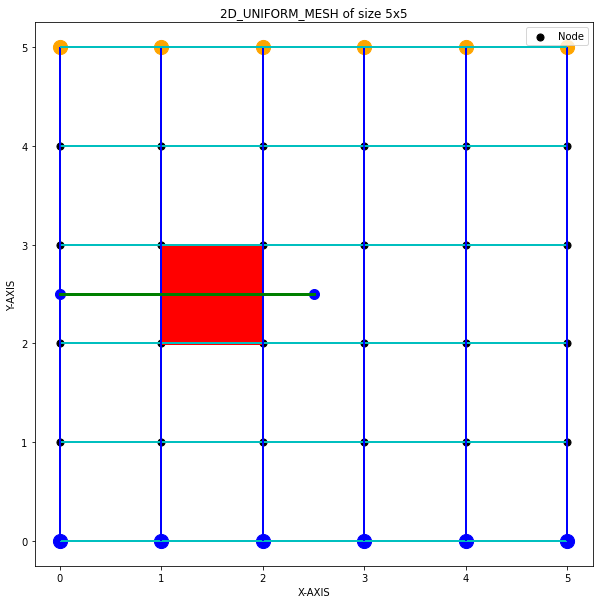
\includegraphics[scale=0.4]{pretip.png}
  \textbf{\caption{Mixed enriched element}}
\end{figure}

\subsection{\color{Black} {Heaviside step function}}
The function usually takes the value of either +1 or 0 based on the function evaluated. the illustration is shown below. For an element completely cut by the crack, Heaviside function takes the value of +1, if the Gauss point is above the crack segment and -1 if the Gauss point is below the crack segment and will be 0 if it is lying on the crack segment. The step function is easy to calculate based on the sign of the $\Delta$. One of the easiest ways is the Orientation test\cite{ahmed2009extended}.\\

\begin{figure}[h]
    \centering
    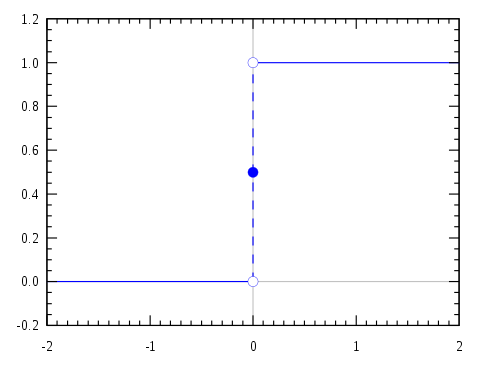
\includegraphics[scale =0.5]{Hside.png}
    \textbf{\caption{Blended-elements}} \cite{ahmed2009extended}
    \centering
\end{figure}

$$
H(x)\cite{ahmed2009extended} = 
\left\{
\begin{array}{ll}
+1 & sign\lVert \Delta \rVert > 0\\
\tab[0.1cm] 0 & sign\lVert \Delta \rVert = 0\\
-1 & sign\lVert \Delta \rVert < 0\\
\end{array}
\right.
$$
$\lVert \Delta \rVert$, represents the determinant value of the matrix $\Delta$ which is calculated using orientation test

\subsection{\color{Black} {Orientation test}}
Orientation test determines whether the point under consideration is above or below the given line segments. The test is performed by evaluating a sign of the determinant. We formulate a triangle using 2 points from the crack segment and 1 query point and evaluating determinant will give the twice the area of a triangle. \newline

It is obvious that, if the a triangle is formed above the crack segment, the sign of the determinant will be positive and should the triangle is formed below the crack segment, the sign of the determinant will be negative, and if the query point falls on the line, the determinant will have a zero value. Mathematically it can be expressed as:

\begin{figure}[h]%
    \centering
    \subfloat[\centering Query point "c" above]{{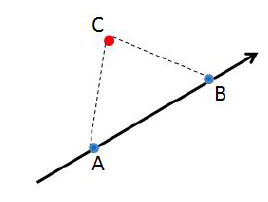
\includegraphics[width=7cm]{LHS.png}}}\hspace{1.5cm}
    \subfloat[\centering Query point "c" below]
    {{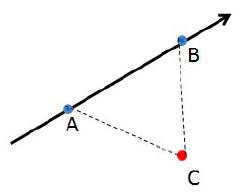
\includegraphics[width=7cm]{RHS.png}}}%
    \textbf{\caption{Orientation test}}\cite{ahmed2009extended}%
\end{figure}

$$
\Delta \cite{ahmed2009extended} =  
\begin{bmatrix}
a_x - c_x & a_y - c_y\\
b_x - c_x & b_y - c_y\\
\end{bmatrix}
$$\newline
In the above matrix, 'a' and 'b' are the coordinates of the crack segment and 'c' is the coordinates of the point under query.
This methodology is applied for all the crack segments in a loop and the determinant value which has the least magnitude will be considered and the sign of that value is calculated.

\subsection{\color{Black} {Heaviside Enrichment}}
The nodes or elements that are enriched using Heaviside step function are called Heaviside enriched node or element. Each node that is Heaviside enriched will have 2 additional DOFs. Suppose all the nodes of the element are Heaviside enriched then the element will have a 16x16 element stiffness matrix. Below figure shows which element has been chosen for the heaviside enrichment.

\begin{figure}[h]
    \centering
    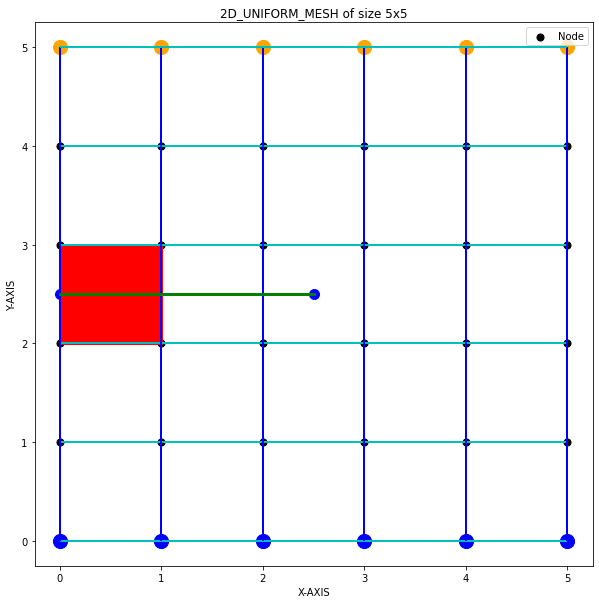
\includegraphics[scale =0.5]{Heavy_enr.png}
    \textbf{\caption{Heaviside enriched element}}
    \centering
\end{figure}

\subsection{\color{Black} {Near-tip enrichment functions}}
This is one of the extrinsic enrichment functions, which is used to enrich an element containing the crack tip. Branch functions are derived from the analytical solution using linear elastic fracture mechanics theory, and they are given as \newline

$$\beta_{\alpha}\cite{pandey2019new} = \left\{\beta_1, \beta_2, \beta_3, \beta_4 \right\} = \sqrt r \left[\cos\frac{\theta}{2}, \sin\frac{\theta}{2}, \cos\frac{\theta}{2} \sin{\theta}, \sin\frac{\theta}{2} \sin\theta \right]$$
\newpage

\begin{figure}[h]
    \centering
    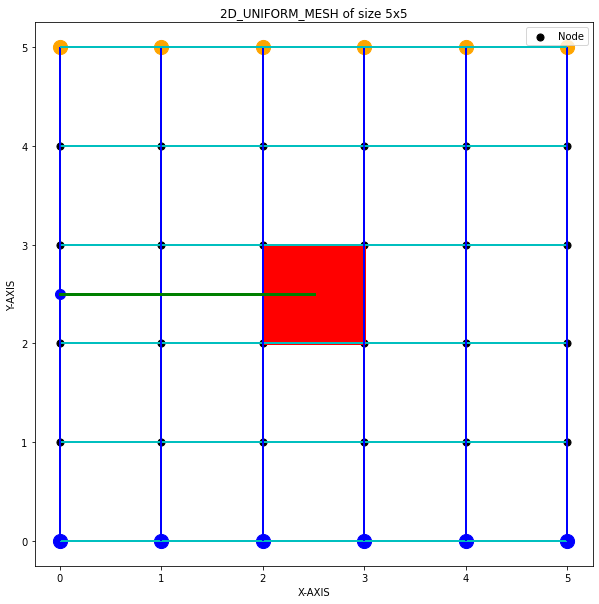
\includegraphics[scale =0.55]{Tip_enr.png}
    \textbf{\caption{Tip enriched element}}
    \centering
\end{figure}

It should be mentioned here that $r$ and $\theta$ are in polar coordinates w.r.t crack tip.
$r$ is the distance measure from the point of the query to the crack tip Ex:\space Node to crack tip, Gauss point to crack tip. It is vital to mention here that the distance measured, $r$, should be transformed from global coordinate system to crack tip coordinate system.
$$
\begin{bmatrix} X_{ctcs} \\ Y_{ctcs}  \end{bmatrix}
=
\begin{bmatrix}
\cos\alpha & \sin\alpha\\
-\sin\alpha & \cos\alpha\\
\end{bmatrix}
*
\begin{bmatrix}
x_{global} - X_{tip}\\
y_{global} - Y_{tip}\\
\end{bmatrix}
$$

$$r = \sqrt{X_{ctcs}^2 + Y_{ctcs}^2} \tab \theta = \arctan\left[\frac{Y_{ctcs}}{X_{ctcs}}\right]
$$
$\alpha$ is the angle made by the crack w.r.t x-axis, $\theta$ should lie in the range of $0$ to $\pm \pi$, 'ctcs' is defined as crack tip coordinate system.\par
The nodes that are enriched using Near-tip enrichment functions are called tip enriched nodes/elements will have 8 additional DOFs these nodes are called Tip enriched nodes. The above figure properly illustrates the scenario. Suppose all the nodes of the element are Tip enriched then the element stiffness matrix will have a size 40x40 for the corresponding element. (8-classical DOFs, $\beta_1- 8 DOFs, \beta_2- 8 DOFs, \beta_3- 8 DOFs, \beta_4- 8 DOFs = 40 DOFs)$

\subsection{\color{Black} {Derivatives of the near-tip enrichment functions}}
The near-tip enrichment functions are represented in local polar coordinates and hence it has to be transformed to global Cartesian coordinate system. The derivatives of the enrichment functions with regard to global coordinates can be evaluated using the chain rule \cite{mohammadi2008extended} 

$$\dv{F}{X} = \pdv{F}{r} \cdot \pdv{r}{X} + \pdv{F}{\theta} \cdot \pdv{\theta}{X}$$
$$\dv{F}{Y} = \pdv{F}{r} \cdot \pdv{r}{Y} + \pdv{F}{\theta} \cdot \pdv{\theta}{Y}$$ 
Derivatives of F$\alpha$ ($r$,$\theta$) with respect to the crack tip polar coordinates ($r$,$\theta$) become

$$F_{1,r} = \frac{1}{2\sqrt r} \sin\frac{\theta}{2}, \tab[0.45cm] F_{1,\theta} = \frac{\sqrt r}{2} \cos\frac{\theta}{2}$$

$$F_{2,r} = \frac{1}{2\sqrt r} \cos\frac{\theta}{2}, \tab[0.45cm] F_{2,\theta} = -\frac{\sqrt r}{2} \sin\frac{\theta}{2}$$

$$F_{3,r} = \frac{1}{2\sqrt r} \sin\frac{\theta}{2} \sin\theta, \tab[0.45cm] F_{3,\theta} = \sqrt r \left[\frac{1}{2}\cos\frac{\theta}{2} \sin\theta + \sin\frac{\theta}{2} \cos\theta \right]$$

$$F_{4,r} = \frac{1}{2\sqrt r} \cos\frac{\theta}{2} \sin\theta, \tab[0.45cm] F_{4,\theta} = \sqrt r \left[-\frac{1}{2}\sin\frac{\theta}{2} \sin\theta + \cos\frac{\theta}{2} \cos\theta \right]$$
\newline
and the derivatives of {$F_\alpha$} ($r$,$\theta$)\cite{mohammadi2008extended} with respect to the local crack coordinate system $(x', y')$ can then be defined as:

$$F_{1,x'} = -\frac{1}{2\sqrt r} \sin\frac{\theta}{2}, \tab[0.45cm] F_{1,y'} = \frac{1}{2\sqrt r} \cos\frac{\theta}{2}$$

$$F_{2,x'} = \frac{1}{2\sqrt r} \cos\frac{\theta}{2}, \tab[0.45cm] F_{2,y'} = \frac{1}{2\sqrt r} \sin\frac{\theta}{2}$$

$$F_{3,x'} = -\frac{1}{2\sqrt r} \sin\frac{3\theta}{2} \sin\theta, \tab[0.45cm] F_{3,y'} = \frac{1}{2\sqrt r} \left[\sin\frac{\theta}{2} + \sin\frac{3\theta}{2} \cos\theta \right]$$

$$F_{4,x'} = -\frac{1}{2\sqrt r} \cos\frac{3\theta}{2} \sin\theta, \tab[0.45cm] F_{4,y'} = \frac{1}{2\sqrt r} \left[\cos\frac{\theta}{2} + \cos\frac{3\theta}{2} \cos\theta \right]$$\newline

Finally, the derivatives of the asymptotic functions $F_{\alpha}$ \cite{mohammadi2008extended} in the global coordinate system are obtained by using the below equations.
$$\pdv{r}{X} = \pdv{r}{x} \cdot \pdv{x}{X} + \pdv{r}{y} \cdot \pdv{y}{X}; \tab[0.45cm] \pdv{r}{Y} = \pdv{r}{x} \cdot \pdv{x}{Y} + \pdv{r}{y} \cdot \pdv{y}{X}$$

$$\pdv{\theta}{X} = \pdv{\theta}{x} \cdot \pdv{x}{X} + \pdv{\theta}{y} \cdot \pdv{y}{X}; \tab[0.45cm] \pdv{\theta}{Y} = \pdv{\theta}{x} \cdot \pdv{x}{Y} + \pdv{\theta}{y} \cdot \pdv{y}{Y}$$\newline
where the derivatives of $r$ and $\theta$ w.r.t to x,y \cite{mohammadi2008extended} can be written as\newline
$$\pdv{r}{x} = \cos\theta \tab[0.45cm] \pdv{\theta}{x} = -\frac{\sin\theta}{r}$$
$$\pdv{r}{y} = \sin\theta \tab[0.45cm] \pdv{\theta}{y} = \frac{\cos\theta}{r}$$\newline 
Using the transformation relationship between the global and crack tip coordinates we have\newline
$$\pdv{x}{X} = \cos\alpha, \tab[0.45cm] \pdv{x}{Y} = \sin\alpha$$
$$\pdv{y}{X} = -\sin\alpha, \tab[0.45cm] \pdv{y}{Y} = \cos\alpha $$


\section{\color{Black} \large{Formulation of XFEM shape functions and B-matrix in the framework of FEM}}

Construction of XFEM shape function N and strain-displacement matrix B is straight forward. This section comprises of the detailed information regarding the generation of N and B matrices.

$$
[B] = 
\begin{bmatrix}
B_{STD} & B_{enr}
\end{bmatrix}
$$

$$
[N] = 
\begin{bmatrix}
N_{STD} & N_{enr}
\end{bmatrix}
$$

\subsection{\color{Black} { Shape functions}}

\begin{figure}[h]
    \centering
    \includegraphics[scale = 1.5]{iso.png}
    \textbf{\caption{Iso Parametric Element}}\cite{sukumar2003modeling}
    \centering
\end{figure}

The shape functions that are used in XFEM are same as the shape functions used in FEM. For a four noded iso-parametric quadrilateral element, the standard FEM bi-linear shape functions \cite{khoei2014extended}associated with each node are given as%

$$N1 = (1-\xi_1)(1-\xi_2) ; \tab[0.45cm] N2 = (1+\xi_1)(1-\xi_2)$$
$$N3 = (1+\xi_1)(1+\xi_2) ; \tab[0.45cm] N4 = (1-\xi_1)(1+\xi_2)$$

The displacement approximation \cite{khoei2014extended} can then be written as
$$
u(X) = \large \begin{bmatrix}
N1 & 0 & N2 & 0 & N3 & 0 & N4 & 0\\
0 & N1 & 0 & N2 & 0 & N3 & 0 & N4\\
\end{bmatrix} \large
\cdot
\large \begin{bmatrix}
u_{x1}\\
u_{y1}\\
u_{x2}\\
u_{y2}\\
u_{x3}\\
u_{y3}\\
u_{x4}\\
u_{y4}\\
\end{bmatrix} \large
= N_{std}u
$$

Where $u$ represents displacements of the given element. Each node has 2 DOFs hence the displacement matrix has a shape of 8x1. The standard FEM shape function matrix is given as

$$
N_{STD} = \large \begin{bmatrix}
N1 & 0 & N2 & 0 & N3 & 0 & N4 & 0\\
0 & N1 & 0 & N2 & 0 & N3 & 0 & N4\\
\end{bmatrix} \large
$$
\newline
for a generic enrichment function g(X), the enriched shape function matrix\cite{khoei2014extended} will be
$$
N_{ENR} = \large \begin{bmatrix}
(N_1g),x & 0 & (N_2g),x & 0 & (N_3g),x & 0 & (N_4g),x & 0 \\
0 & (N_1g),y & 0 & (N_2g),y & 0 &(N_3g),y & 0 & (N_4g),y\\
\end{bmatrix} \large
$$
The shape functions are in local coordinate system and it should be transformed into global coordinate system. This is accomplished by using Jacobian \cite{khoei2014extended} and the steps are as follows
\begin{itemize}
    \item Take the derivatives of the shape functions w.r.t $\xi_1$ and $\xi_2$
    $$N_{1,\xi_1}= -\frac{1}{4}(1-\xi_2), \tab[0.25cm] N_{1,\xi_2}= - \frac{1}{4}(1-\xi_1)$$
    $$N_{2,\xi_1}=  \frac{1}{4}(1-\xi_2),  \tab[0.25cm] N_{2,\xi_2}= - \frac{1}{4}(1+\xi_1)$$
    $$N_{3,\xi_1}=  \frac{1}{4}(1+\xi_2),  \tab[0.25cm] N_{3,\xi_2}=  \frac{1}{4}(1+\xi_1)$$
    $$N_{4,\xi_1}= -\frac{1}{4}(1+\xi_2), \tab[0.25cm] N_{4,\xi_2}=  \frac{1}{4}(1-\xi_1)$$
    
    $$
    \pdv{[N]}{\xi} = \large \begin{bmatrix} 
    \dv{N_i} {\xi_1} \\[7pt]
    \dv{N_i} {\xi_2} \\
    \end{bmatrix} \large
    =
    \begin{bmatrix}
    -(1-\xi_2) & 1-\xi_2 & 1+\xi_2 & -(1+\xi_2) \\
    -(1-\xi_1) & -(1+\xi_1) & 1+\xi_1 & 1 - \xi_1 \\
    \end{bmatrix}
    $$
    \item Multiply the derivatives with the corresponding nodal coordinates this gives the Jacobi matrix of 2x2.
    $$
    J = \pdv{[N]}{\xi} \cdot (X^e)^T \\
    $$
    \item Take the inverse of the Jacobi matrix
    \item Multiply the inverse of the Jacobi matrix with the differentiated shape functions from step 1 generating a 2x4 matrix.
    $$
    \pdv{[N]}{x} = J^{-1} \cdot \pdv{[N]}{\xi}
    $$
    \item The elements in this matrix are arranged in a specified manner to get B-matrix.  
    
\end{itemize}
\subsection{\color{Black} {B-matrix}}
This is also called as a Strain-Displacement matrix which gives a relation between strains and displacements\cite{khoei2014extended}.

$$
B_{std} = \begin{bmatrix}
N_{1,x} & 0 & N_{2,x} & 0 & N_{3,x} & 0 & N_{4,x} & 0 \\
0 & N_{1,y} & 0 & N_{2,y} & 0 & N_{3,y} & 0 & N_{4,y}\\
N_{1,y} & N_{1,x} & N_{2,y} & N_{2,x} & N_{3,y} & N_{3,x} & N_{4,y} & N_{4,x}
\end{bmatrix}
$$
\newline
Enriched B-matrix \cite{khoei2014extended} is given by
$$
B_{enr} = \begin{bmatrix}
(N_1g),x & 0 & (N_2g),x & 0 & (N_3g),x & 0 & (N_4g),x & 0 \\
0 & (N_1g),y & 0 & (N_2g),y & 0 &(N_3g),y & 0 & (N_4g),y\\
(N_4g),y & (N_1g),x & (N_4g),y & (N_4g),x & (N_4g),y & (N_4g),x & (N_4g),y & (N_4g),x
\end{bmatrix}
$$
$g(x)$ could be either Heaviside step function or Near Tip function. The below table gives the information on the additional degrees of freedom generated due to the enrichment
\newline

\begin{tabularx}{1\textwidth} { 
  | > {\centering\arraybackslash}X 
  | >{\centering\arraybackslash}X  
  | >{\centering\arraybackslash}X | }
  
 \hline
 \textbf {g(x)} & \textbf {Enrichment type} & \textbf {Degrees of freedom}\\
 \hline
 H(X) & Heaviside function or Heaviside step function & 2 DOFs per node\\
\hline
 $F^4 (r,\theta) $  & near-tip enrichment function & 8 DOFs per node\\
 \hline
\end{tabularx}\newline

If the node is Heaviside enriched, the B-matrix\cite{khoei2014extended} is given by
$$
B_{Heavy} = \begin{bmatrix}
(N_i H(x))_x & 0\\
0 & (N_i H(x))_y\\
(N_i H(x))_y & (N_i H(x))_x
\end{bmatrix}
\: i=1,2,3,4
$$
The derivative of Heaviside function is the Dirac delta function\cite{khoei2014extended}, that is
$$(N_i H(x))_x = N_{i,x} H_{,x}(x) = \delta$$
If the node is tip enriched, the B-matrix \cite{khoei2014extended} is given by
$$
B_{tip} = \begin{bmatrix}
(N_i F_{\alpha})_,x & 0\\
0 & (N_i F_{\alpha})_,y\\
(N_i F_{\alpha})_,y & (N_i F_{\alpha})_,x\\
\end{bmatrix}
\: \alpha = 1,2,3,4
$$
The derivative of near-tip enrichment function\cite{khoei2014extended} is given by
$$(N_i F_{\alpha})_,x = F_{\alpha} N_{i,x} + F_{\alpha,x} N_i ; \tab[1cm] (N_i F_{\alpha})_,y = F_{\alpha} N_{i,y} + F_{\alpha,y} N_i $$

when $i=1, \alpha = 1,2,3,4$
$$(N_1 F_1)_,x = F_1 N_{1,x} + F_{1,x} N_1 $$
$$(N_1 F_2)_,x = F_2 N_{1,x} + F_{2,x} N_1 $$
$$(N_1 F_3)_,x = F_3 N_{1,x} + F_{3,x} N_1 $$
$$(N_1 F_4)_,x = F_4 N_{1,x} + F_{4,x} N_1 $$

Then the tip enriched B-matrix for 1 node is represented as,
$$
B_{tip} = \begin{bmatrix}
F_1 N_{1,x} + F_{1,x} N_1 & 0 & \dots  & F_4 N_{1,x} + F_{4,x} N_1 & 0\\
0 & F_1 N_{1,y} + F_{1,y} N_1 & \dots & 0 & F_4 N_{1,y} + F_{4,y} N_1\\
F_1 N_{1,y} + F_{1,y} N_1 & F_1 N_{1,x} + F_{1,x} & \dots & F_4 N_{1,y} + F_{4,y} N_1 & F_4 N_{1,x} + F_{4,x} N_1\\
\end{bmatrix}
\: \alpha = 1,2,3,4
$$

the same has to be implemented for the other 3 nodes if all 4 nodes in the element are tip enriched.

\subsection{\color{Black} {Numerical Integration}}

In the classical FEM, the standard shape functions are of the polynomial order and the Gauss integration rule can be used to evaluate the integral of stiffness matrix. However, in the X-FEM the enriched shape functions are obtained in terms of non-polynomial order. Moreover, the enrichment functions may not be smooth over an enriched element due to presence of the weak or strong discontinuity inside the element. Hence, the standard Gauss quadrature rule cannot be used if an element is crossed over by a crack, and necessary modifications are necessary for numerical integration over an enriched element\cite{khoei2014extended}. \par

The suggested approach is based on the increase of the
number of Gauss integration points\cite{khoei2014extended}, as shown in the below Figure, however, this  may also result in a substantial loss of accuracy. In order to overcome these difficulties, the enriched element will be divided into n-number of sub-polygons 
as shown in Figure, and the Gauss integration rule is performed over each sub-polygons. The sub-polygons do not produce additional DOFs\cite{khoei2014extended}. In the end all the K-matrices of the sub polygons will be summed up to get a K-matrix of the corresponding element.\par
Consider an element cut by an interface into two distinct parts, $\Omega+$ and $\Omega-$; the integration of stiffness matrix  over a domain (element) $\Omega$ can be performed as

\begin{figure}[H]
    \centering
    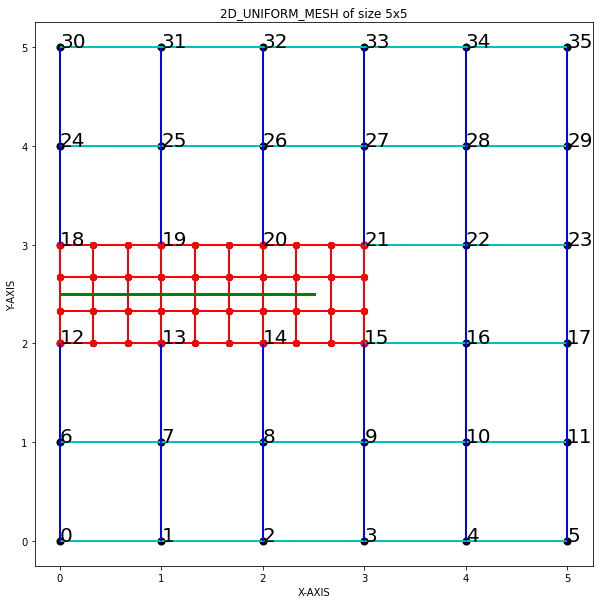
\includegraphics[scale =0.5]{Subdivision.png}
    \textbf{\caption{9 Sub-polygons per element}}
    \centering
\end{figure}


$$\enspace K_{ij}^{\alpha\beta} = \int_{\Omega} B_{i(\xi_1,\xi_2)}^T*D*B_{j(\xi_1,\xi_2)}*\lVert J \rVert d\xi_1d\xi_2$$\vspace{0.1cm}
$$ = \int_{\Omega+} B_{i(\xi_1,\xi_2)}^T*D*B_{j(\xi_1,\xi_2)}*\lVert J \rVert d\xi_1d\xi_2 + \int_{\Omega-} B_{i(\xi_1,\xi_2)}^T*D*B_{j(\xi_1,\xi_2)}*\lVert J \rVert d\xi_1d\xi_2 $$\vspace{0.1cm}
$$= \sum_{l=1}^{\mathscr{N}^{SUB+}} \left(\sum_{k=1}^{\mathscr{N}^{GP+}} B_{i(\xi_{1k},\xi_{2k})}^T*D*B_{j(\xi_{1k},\xi_{2k})}*w_k \right)_l  + \sum_{l=1}^{\mathscr{N}^{SUB-}} \left(\sum_{k=1}^{\mathscr{N}^{GP-}} B_{i(\xi_{1k},\xi_{2k})}^T*D*B_{j(\xi_{1k},\xi_{2k})}* w_k \right)_l $$\vspace{0.1cm}

where in ${\mathscr{N}^{SUB+}}$ and ${\mathscr{N}^{SUB-}}$ are the number of sub-polygons in $\Omega+$ and $\Omega-$, and ${\mathscr{N}^{GP+}}$ and ${\mathscr{N}^{GP-}}$ are the number of Gauss points at each sub-polygon in $\Omega+$ and $\Omega-$, respectively.In this relation, $w_k$ is the weight of quadrature point. Therefore, Gauss quadrature can be employed, which allows integration of polynomials up to a certain order in the given element. 

\subsection{\color{Black} {Element connectivity matrix}}
The matrix which is used to assemble all the element stiffness matrix. The matrix consists of only 0s and 1s. The size of the connectivity matrix is decided based on the number of DOFs available in the geometry. The columns of the matrix is the maximum DOFs available in the geometry and the rows of the matrix is the maximum DOFs available in the single element. As mentioned in the previous section, the additional DOFs will be placed after allotting rows and columns for normal DOFs.  

$A_{matrix} = [Max DOFs availabe in per element] X [Max DOFs availabe in the geometry]$ 

\subsection{\color{Black} {Element stiffness matrix}}
The element stiffness matrix for classical element is given by \cite{khoei2014extended}
$$ K = \int_{-1}^{1} \int_{-1}^{1} B_{\xi_1, \xi_2}^T*D*B_{\xi_1, \xi_2}*\lVert J \rVert d\xi_1d\xi_2 $$
The BVP is solved using
    $$ [K][u] = [F]$$

Wherein \newline
\tab[1cm] K = $K_{global}$, is called the global stiffness matrix\newline
\tab[1cm] u = Displacement matrix\newline
\tab[1cm] F = Force vector

\subsection{\color{Black} {Nodal Displacements}}
After solving BVP, a 1D displacement vector is obtained. This vector contains both classical and enriched displacements. It should be noted that if there a node is enriched, then displacement of that node will be summed with the enriched displacements and multiplied with the enrichment function value. Using the displacement approximation equation, corresponding nodal displacements are calculated. The relation handles both classical and enriched displacements.

$$u(x) = \sum_{i=1}^n N_i(x)u_i + \sum_{j^{heavy}=1}^P N_j(x)[\psi(x)] a_j + \sum_{k^{tip}=1}^4 N_k(x)[\beta_{\alpha}(x)] b_{k^\alpha} $$

The displacements that are calculated using XFEM should be treated the same way as the stresses. But before transforming, one should calculate the gradient of the XFEM displacements \cite{ahmed2009extended} and it is given by
\vspace{-0.1cm}
$$
 \begin{bmatrix}
u_{x(XFEM)} & u_{y(XFEM)}\\
v_{x(XFEM)} & v_{y(XFEM)}\\
\end{bmatrix}
=
B_{std} = \begin{bmatrix}
N_{1,x} & 0 & N_{2,x} & 0 & N_{3,x} & 0 & N_{4,x} & 0 \\
0 & N_{1,y} & 0 & N_{2,y} & 0 & N_{3,y} & 0 & N_{4,y}\\
\end{bmatrix}
*
\large \begin{bmatrix}
u_{x1}\\
u_{y1}\\
u_{x2}\\
u_{y2}\\
u_{x3}\\
u_{y3}\\
u_{x4}\\
u_{y4}\\
\end{bmatrix} \large
$$

Transformation of displacement gradients to crack tip coordinate system
$$
\begin{bmatrix}
U_{X (CTCS)} & U_{Y (CTCS)}\\
V_{X (CTCS)} & V_{Y (CTCS)}\\
\end{bmatrix}
=
\begin{bmatrix}
\cos\alpha & \sin\alpha\\
-\sin\alpha & \cos\alpha\\
\end{bmatrix}
*
\begin{bmatrix}
u_{x (XFEM)} & u_{y (XFEM)}\\
v_{x (XFEM)} & v_{y (XFEM)}\\
\end{bmatrix}
*
\begin{bmatrix}
\cos\alpha & -\sin\alpha\\
\sin\alpha & \cos\alpha\\
\end{bmatrix}
$$

\subsection{\color{Black} {Calculation of Stresses and Strains}}
After the computation of displacements, strains must be calculated using strain-displacement matrix (B-matrix) and it is given by

$$\epsilon = [B][u]$$
\vspace{-0.3cm}
$$
\begin{bmatrix}
\epsilon_x\\
\epsilon_y\\
\gamma_{xy}\\
\end{bmatrix}
=
\begin{bmatrix}
N_{1,x} & 0 & N_{2,x} & 0 & N_{3,x} & 0 & N_{4,x} & 0 \\
0 & N_{1,y} & 0 & N_{2,y} & 0 & N_{3,y} & 0 & N_{4,y}\\
N_{1,y} & N_{1,x} & N_{2,y} & N_{2,x} & N_{3,y} & N_{3,x} & N_{4,y} & N_{4,x}
\end{bmatrix}
*
\large \begin{bmatrix}
u_{x1}\\
u_{y1}\\
u_{x2}\\
u_{y2}\\
u_{x3}\\
u_{y3}\\
u_{x4}\\
u_{y4}\\
\end{bmatrix} \large
$$
wherein $\epsilon$ is the strain and B is B-matrix and u is the nodal displacements.
\newline
Stresses are calculated using the relation
$$\sigma = [D][\epsilon]$$
$$
\begin{bmatrix}
\sigma_x\\
\sigma_y\\
\sigma_{xy}\\
\end{bmatrix}
=
\frac{E}{1-\nu^2}
\begin{bmatrix}
1 & \nu & 0\\
\nu & 1 & 0\\
0 & 0 & \frac{1-\nu}{2}\\
\end{bmatrix}
*
\begin{bmatrix}
\epsilon_x\\
\epsilon_y\\
\gamma_{xy}\\
\end{bmatrix}
$$

The stresses that are calculated using XFEM should be transformed from global coordinate system to crack tip coordinate system using appropriate rotation matrix \cite{ahmed2009extended} and the equation is given by\vspace{0.1cm}
$$
\begin{bmatrix}
\sigma_{XX (CTCS)} & \sigma_{XY (CTCS)}\\
\sigma_{XY (CTCS)} & \sigma_{YY (CTCS)}\\
\end{bmatrix}
=
\begin{bmatrix}
\cos\alpha & \sin\alpha\\
-\sin\alpha & \cos\alpha\\
\end{bmatrix}
*
\begin{bmatrix}
\sigma_{xx (XFEM)} & \sigma_{xy (XFEM)}\\
\sigma_{yx (XFEM)} & \sigma_{yy (XFEM)}\\
\end{bmatrix}
*
\begin{bmatrix}
\cos\alpha & -\sin\alpha\\
\sin\alpha & \cos\alpha\\
\end{bmatrix}
$$\vspace{0.1cm}

%===============================================================================
\section{\color{Black} \large{Linear Elastic Fracture mechanics}}
\subsection{\color{Black}{Introduction}}

Strength of the materials were computed in the past based on two possible theories [Griffith 1921]. A material is said to fracture if maximum tensile stress or maximum extension in a body exceeds a certain threshold value\cite{kuna2013finite}. Hence the strength of the material is basically considered to be an intrinsic property. \newline

One of earliest recorded incidents of brittle fracture failure was the Montrose bridges 1830 [Erdogan 2000]. There have been many incidents due to fracture failure after that e.g the event of Tay Rail Bridge failure in 1879 \cite{kuna2013finite}. These incidents led the scientists and engineers to exploit the Fracture mechanics domain. \newline

It is said that Griffith’s and Irwin’s work has led the foundations for a new engineering branch “Engineering Fracture Mechanics” to flourish, and soon after that Fracture mechanics evolved as an important branch in the engineering realm. 
A very good review on fracture mechanics can be found in Erdogan [2000]. More details on engineering fracture mechanics can also be found in \cite{kuna2013finite}

\subsection{\color{Black}{Modes of Failure}}
Failure is defined as the rupture of the sample under the applied load. There are three modes of failure, namely Mode I, Mode II, and Mode III \cite{kuna2013finite}.
\begin{itemize}
    \item Mode I: is the opening type wherein a tensile load is applied normal to the crack surfaces and crack opens perpendicular to the crack plane i.e. the crack propagation angle is 0.
    \item Mode II: A shear load is applied parallel to the crack surfaces and the crack is allowed to propagate. The crack propagation angle varies from +70 degrees to -70 degrees. The crack faces are found to be sliding in the direction of applied load.
    \item Mode III, a shear stress is applied perpendicular to the plane of the crack. This is also called as Out-of-plane tearing mode.
\end{itemize}
The three modes of failures are shown schematically in the below figures.

\begin{figure}[H]
  \begin{minipage}[b]{0.4\textwidth}
    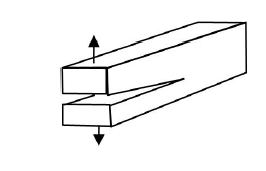
\includegraphics[scale = 0.8]{M1.png}
    \textbf{\caption{{Mode-I Type failure \cite{kuna2013finite}}}}
  \end{minipage}
  \hspace{2cm}
  \begin{minipage}[b]{0.4\textwidth}
    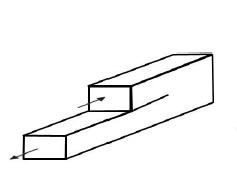
\includegraphics[scale = 0.8]{M2.png}
    \textbf{\caption{{Mode-II Type failure \cite{kuna2013finite}}}}
  \end{minipage}
\end{figure}

\begin{figure}[h]
    \centering
    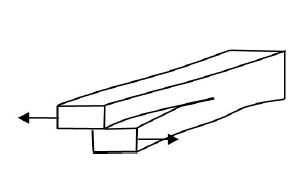
\includegraphics[scale = 0.8]{M3.png}
    \textbf{\caption{{Mode-III Type failure \cite{kuna2013finite}}}}
    \centering
\end{figure}

\section{\color{Black} \large{Displacement and Stress Fields at the Crack Tip Area}}

The importance of stress singularity at the crack tip area was presented by Westergard (1939) and Williams (1957) by evaluation of the displacement and stress fields around the crack tip area. Williams (1957) used the Airy stress function to capture the singularity at the crack tip area using a polar coordinate system \cite{khoei2014extended} $(r, \theta)$ as

$$\Phi = r^{\lambda+1} (c_1 \sin(\lambda+1)\hat{\theta} + c_2 \cos(\lambda+1)\hat{\theta} + c_3 \sin(\lambda-1)\hat{\theta} + c_4 \sin(\lambda-1)\hat{\theta})$$

wherein $c_i$ are the coefficients and $\hat{\theta}$ is depicted in the below Figure
\begin{figure}[h]
    \centering
    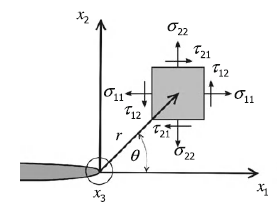
\includegraphics[scale = 1]{stress.PNG}
    \textbf{\caption{{Stresses at the crack tip in Cartesian coordinates     \cite{kuna2013finite}}}}
    \centering
\end{figure}
%-------------------------------------------------------------------------------------
\subsection{\color{Black}{Auxiliary displacements for mode-I}}
Substituting the Airy stress function EQUATION in the equilibrium equation of the system, that is , $\bigtriangledown^2 \bigtriangledown^2\Phi = 0$ \cite{khoei2014extended}
in the absence of body forces, applying the traction-free boundary conditions at the crack faces. It should be noted here that the displacement field is a function of crack tip polar coordinate system and we are required to find the spatial derivatives according to the local crack tip Cartesian coordinate system \cite{nagashima2003stress}. This will be evaluated as follows

$$U_x = \frac{K_I (1+\nu)}{E} \sqrt{\frac{r}{2\pi}} \cos\frac{\theta}{2} \left[k-1+2\sin^2\frac{\theta}{2} \right]$$\vspace{0.1cm}
$$U_y = \frac{K_I (1+\nu)}{E} \sqrt{\frac{r}{2\pi}} \sin\frac{\theta}{2} \left[k+1-2\cos^2\frac{\theta}{2} \right]$$\vspace{0.1cm}
$$U_z = 0$$

Derivatives of the displacement $U_x$ and $U_y$ w.r.t to $x$ and $y$ \cite{nagashima2003stress} is given as

$$\dv{U_x}{X} = \dv{U_x}{r}*\dv{r}{X} + \dv{U_x}{\theta}*\dv{\theta}{X} \tab[1cm] \dv{U_x}{Y} = \dv{U_x}{r}*\dv{r}{Y} + \dv{U_x}{\theta}*\dv{\theta}{Y}$$

$$\dv{U_y}{X} = \dv{U_y}{r}*\dv{r}{X} + \dv{U_y}{\theta}*\dv{\theta}{X} \tab[1cm] \dv{U_y}{Y} = \dv{U_y}{r}*\dv{r}{Y} + \dv{U_y}{\theta}*\dv{\theta}{Y}$$\vspace{0.2cm}

Derivatives of the displacement $U_x$ and $U_y$ w.r.t to $r$ and $\theta$ \cite{nagashima2003stress}is given as 
$$\dv{U_x}{r} = \frac{K_I(1+\nu)}{2D} \frac{1}{\sqrt{2\pi r}} \cos\frac{\theta}{2} (k-\cos\theta)$$

$$\dv{U_x}{\theta} = \frac{K_I(1+\nu)}{D} \sqrt{\frac{r}{2\pi}} \left[-0.5\sin\frac{\theta}{2} (k-\cos\theta) + \sin\theta \cos\frac{\theta}{2} \right]$$

$$\dv{U_y}{r} = \frac{K_I(1+\nu)}{2D} \frac{1}{\sqrt{2\pi r}} \sin\frac{\theta}{2} (k-\cos\theta)$$

$$\dv{U_x}{\theta} = \frac{K_I(1+\nu)}{D} \sqrt{\frac{r}{2\pi}} \left[0.5\cos\frac{\theta}{2} (k-\cos\theta) + \sin\theta \sin\frac{\theta}{2} \right]$$\vspace{0.2cm}

Derivatives $r$ and $\theta$ w.r.t to $x$ and $y$ \cite{khoei2014extended} is given by
$$\dv{r}{X} = \cos\theta \tab[1cm] \dv{r}{Y} = \sin\theta$$
$$\dv{\theta}{X} = -\sin\frac{\theta}{r} \tab[1cm] \dv{\theta}{Y} = \cos\frac{\theta}{r}$$
%-------------------------------------------------------------------------------------
\subsection{\color{Black}{Auxiliary stresses for mode-I}}
More information on the Auxiliary stresses for mode-I is available in \cite{khoei2014extended}

$$\sigma_{x} = \frac{K_I}{\sqrt{2\pi r}} \cos\frac{\theta}{2} \left[1-\sin\frac{\theta}{2} \sin\frac{3\theta}{2}\right]$$ 

$$\sigma_{y} = \frac{K_I}{\sqrt{2\pi r}} \cos\frac{\theta}{2} \left[1+\sin\frac{\theta}{2} \sin\frac{3\theta}{2}\right]$$ 

$$\tau_{xy} = \frac{K_I}{\sqrt{2\pi r}} \sin\frac{\theta}{2} \cos\frac{\theta}{2} \cos\frac{3\theta}{2}$$ 

$$
\sigma_{z} = 
\left\{
\begin{array}{ll}
\nu(\sigma_x + \sigma_y) & \mbox{Plane strain}\\
\tab[0.75cm] 0 & \mbox{Plane stress}\\
\end{array}
\right.
$$


%---------------------------------------------------------------------------------------------
\subsection{\color{Black}{Auxiliary displacements for mode-II}}
\vspace{0.5cm}
$$U_x = \frac{K_{II}(1+\nu)}{E} \sqrt{\frac{r}{2\pi}} \sin\frac{\theta}{2} \left[k+1+2\cos^2\frac{\theta}{2} \right]$$\vspace{0.1cm}
$$U_y = \frac{K_{II}(1+\nu)}{E} \sqrt{\frac{r}{2\pi}} \cos\frac{\theta}{2} \left[k-1-2\sin^2\frac{\theta}{2} \right]$$\vspace{0.1cm}
$$U_z = 0$$

Derivatives of the displacement $U_x$ and $U_y$ w.r.t to $r$ and $\theta$ \cite{nagashima2003stress} is given as
$$\dv{U_x}{r} = \frac{K_{II}(1+\nu)}{2D} \frac{1}{\sqrt{2\pi r}} \cos\frac{\theta}{2} (k+2+\cos\theta)$$

$$\dv{U_x}{\theta} = \frac{K_{II}(1+\nu)}{D} \sqrt{\frac{r}{2\pi}} \left[0.5\cos\frac{\theta}{2} (k+2+\cos\theta) - \sin\theta \sin\frac{\theta}{2} \right]$$

$$\dv{U_y}{r} = \frac{K_{II}(1+\nu)}{2D} \frac{1}{\sqrt{2\pi r}} \cos\frac{\theta}{2} (k-2+\cos\theta)$$

$$\dv{U_x}{\theta} = -\frac{K_{II}(1+\nu)}{D} \sqrt{\frac{r}{2\pi}} \left[-0.5\sin\frac{\theta}{2} (k-2+\cos\theta) +- \sin\theta \cos\frac{\theta}{2} \right]$$\vspace{0.2cm}

\subsection{\color{Black}{Auxiliary stresses for mode-II}}\cite{ahmed2009extended}

$$\sigma_{x} = -\frac{K_{II}}{\sqrt{2\pi r}} \sin\frac{\theta}{2} \left[2+\cos\frac{\theta}{2} \cos\frac{3\theta}{2}\right]$$ 

$$\sigma_{y} = \frac{K_{II}}{\sqrt{2\pi r}} \sin\frac{\theta}{2} \cos\frac{\theta}{2} \cos\frac{3\theta}{2}$$ 

$$\tau_{xy} = \frac{K_{II}}{\sqrt{2\pi r}} \cos\frac{\theta}{2} \left[1-\sin\frac{\theta}{2} \sin\frac{3\theta}{2}\right]$$ 

$$
\sigma_{z} = 
\left\{
\begin{array}{ll}
\nu(\sigma_x + \sigma_y) & \mbox{Plane strain}\\
\tab[0.75cm] 0 & \mbox{Plane stress}\\
\end{array}
\right.
$$
Wherein "k" is called Kolosov constant and it is defined as $k=(3-\nu)/(1+\nu)$ for plane stress and $k=3-4\nu$ for plane strain problems and $\nu$ is the Poisson ratio.
\\
In the above relations, $K_{I}$, and $K_{II}$ are the SIFs for mode-I and mode-II respectively and they are given by

$$K_I = \sigma_y \sqrt{2*\pi r} \tab[0.25cm] MPa\sqrt{m}$$
$$K_{II} = \sigma_xy \sqrt{2*\pi r} \tab[0.25cm] MPa\sqrt{m}$$

wherein
\\
\tab[1cm] $\mathbold{\sigma_{x}}$ = Tensile Stress in MPa
\\
\tab[1cm] $\mathbold{\sigma_{xy}}$ = Shear Stress in MPa
\\
\tab[1cm] \textbf{r} = crack length in m

\section{\color{Black} \large{Stress Intensity Factors}}

In the linear elastic fracture mechanics (LEFM), the stress, strain, and displacement fields can be determined by employing the concept of the SIFs near the crack tip region. It is therefore important to accurately evaluate the SIFs for the FE analysis of LEFM.\\

There are many computational algorithms available to evaluate the SIFs. The approaches can be categorized into two groups; the “direct” approach and the “energy” approach. The direct approach relates the SIFs with the FEM results directly, while the energy approach is based on the computation of energy release rate. In general, the energy approaches are more accurate than the direct procedures. However, the direct approaches are more popular and are usually used to verify the results of energy approaches, since their expressions are simple. The most popular energy approach is the J-integral technique\cite{khoei2014extended}. In the following section the J-integral method is discussed in detail

\subsection{\color{Black} \large{J-integral}}
In Fracture mechanics computations, SIFs are the most important fracture parameters used for the determination of mixed-mode near tip stress, strain, and displacement fields. In order to evaluate the SIFs, the area J–integral is defined in relation below, which can be computed over an area of the FE mesh refer to the figure below. In XFEM modeling, the area for the integration is calculated by assuming a virtual circle with a specific radius around the crack tip, and the integration is performed over the elements that lie inside the circle \cite{kuna2013finite}, as shown in Figure 7.16. \newline

\begin{figure}[h]
    \centering
    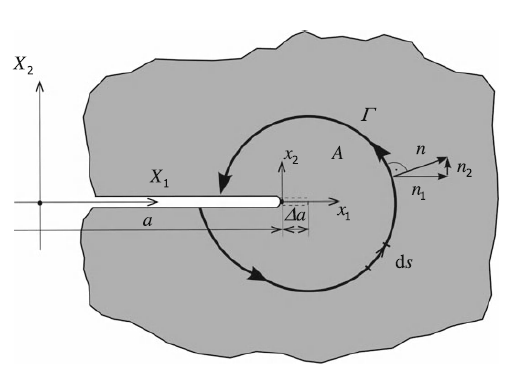
\includegraphics[scale = 1]{J_int.PNG}
    \textbf{\caption{{Elements inside the area are integrated\cite{kuna2013finite}}}}
    \centering
\end{figure}    
    
Basically, J-integral is calculated by adding the integrals computed for a sample without a crack (Auxiliary state / state (2)) and the same sample with crack (current configuration/ state(1)). For this purpose, BVP is solved using XFEM to obtain to obtain the displacement, strain, and stress fields of state (1) that is, $u_i^{(1)}$, $\epsilon_{ij}^{(1)}$, and $\sigma_{ij}^{(1)}$ and these values are then transferred from the global to local crack tip coordinate system $(x_1, x_2)$ by using an appropriate transformation.

$$J = \int_A \left(\sigma_{ij} \pdv{u_i}{x_1} - \mathscr{W}\delta_{ij}\right) \pdv{q}{x_j}dA $$\vspace{0.1cm}
$$ I^{(1,2)} = \int_A \left(- \mathscr{W}^{(1,2)}\delta_{1j} + \sigma_{ij}^{(1)} \pdv{u_i^{(2)}}{x_1} + \sigma_{ij}^{(2)} \pdv{u_i^{(1)}}{x_1}\right) \pdv{q}{x_j}dA $$

Wherein $\mathscr{W}^{(1,2)}$ is the interaction strain energy \cite{kuna2013finite} defined by
$$\mathscr{W}^{(1,2)} = \sigma_{ij}^{(1)} \epsilon_{ij}^{(2)} = \sigma_{ij}^{(2)} \epsilon_{ij}^{(1)}$$

The super scripts $(2)$, and $(1)$ implicates auxiliary state(material without crack) and current state(after the introduction of the crack) respectively.
The distribution of weighting function q in the above relation can be obtained for an element using the standard FE interpolation \cite{kuna2013finite} as

$$q = \sum_{I=1}^{\mathscr{N}^{elem}} N_I(x)q_I $$

where ${\mathscr{N}^{elem}}$ is the number of nodes of an element and $q_I$ are the nodal values of q. The derivation of weighting function can be obtained as

$$\pdv{q}{x} = \sum_{I=1}^{\mathscr{N}^{elem}} \pdv{N_I}{x}q_I $$

After calculating the derivative of the weight function, $\pdv{q}{x}$ is converted to local crack tip coordinate system using appropriate transformation.

$$\left[\pdv{q}{X}\right] = [R] * \left[\pdv{q}{x}\right] $$

where R in the above equation is called rotation matrix and it is defined as:

$$
\large \begin{bmatrix} 
\pdv{q} {X} \\[7pt]
\pdv{q} {Y} \\
\end{bmatrix} \large
=
\begin{bmatrix}
\cos\alpha & \sin\alpha\\
-\sin\alpha & \cos\alpha\\
\end{bmatrix}
*
\large \begin{bmatrix} 
\pdv{q} {x} \\[7pt]
\pdv{q} {y} \\
\end{bmatrix} \large
$$


\newpage
\bibliographystyle{plain}
\bibliography{ref}

\end{document}

